%%%%%%%%%%%%%%%%%%%%%%%%%%%%%%%%%%%%%%%%%
% Short Sectioned Assignment
% LaTeX Template
% Version 1.0 (5/5/12)
%
% This template has been downloaded from:
% http://www.LaTeXTemplates.com
%
% Original author:
% Frits Wenneker (http://www.howtotex.com)
%
% License:
% CC BY-NC-SA 3.0 (http://creativecommons.org/licenses/by-nc-sa/3.0/)
%
%%%%%%%%%%%%%%%%%%%%%%%%%%%%%%%%%%%%%%%%%

%----------------------------------------------------------------------------------------
%	PACKAGES AND OTHER DOCUMENT CONFIGURATIONS
%----------------------------------------------------------------------------------------

\documentclass[paper=a4, fontsize=11pt]{scrartcl} % A4 paper and 11pt font size

\usepackage[T1]{fontenc} % Use 8-bit encoding that has 256 glyphs
\usepackage{fourier} % Use the Adobe Utopia font for the document - comment this line to return to the LaTeX default
\usepackage[english]{babel} % English language/hyphenation
\usepackage{amsmath,amsfonts,amsthm} % Math packages

\usepackage{lipsum} % Used for inserting dummy 'Lorem ipsum' text into the template
\usepackage{graphicx}
\usepackage{float}
\usepackage{sectsty} % Allows customizing section commands
\allsectionsfont{ \normalfont\scshape} % Make all sections centered, the default font and small caps
\usepackage{multirow}

\usepackage{fancyhdr} % Custom headers and footers
\pagestyle{fancyplain} % Makes all pages in the document conform to the custom headers and footers
\fancyhead{} % No page header - if you want one, create it in the same way as the footers below
\fancyfoot[L]{} % Empty left footer
\fancyfoot[C]{} % Empty center footer
\fancyfoot[R]{\thepage} % Page numbering for right footer
\renewcommand{\headrulewidth}{0pt} % Remove header underlines
\renewcommand{\footrulewidth}{0pt} % Remove footer underlines
\setlength{\headheight}{13.6pt} % Customize the height of the header

\numberwithin{equation}{section} % Number equations within sections (i.e. 1.1, 1.2, 2.1, 2.2 instead of 1, 2, 3, 4)
\numberwithin{figure}{section} % Number figures within sections (i.e. 1.1, 1.2, 2.1, 2.2 instead of 1, 2, 3, 4)
\numberwithin{table}{section} % Number tables within sections (i.e. 1.1, 1.2, 2.1, 2.2 instead of 1, 2, 3, 4)

\setlength\parindent{0pt} % Removes all indentation from paragraphs - comment this line for an assignment with lots of text

%----------------------------------------------------------------------------------------
%	TITLE SECTION
%----------------------------------------------------------------------------------------

\newcommand{\horrule}[1]{\rule{\linewidth}{#1}} % Create horizontal rule command with 1 argument of height

\title{	
\normalfont \normalsize 
\textsc{CS 646 - IR} \\ [25pt] % Your university, school and/or department name(s)
\horrule{0.5pt} \\[0.4cm] % Thin top horizontal rule
\huge P3 \\ % The assignment title
\horrule{2pt} \\[0.5cm] % Thick bottom horizontal rule
}

\author{Patrick Verga} % Your name

\date{\normalsize\today} % Today's date or a custom date

\begin{document}

\maketitle % Print the title

%----------------------------------------------------------------------------------------
%	PROBLEM 1
%----------------------------------------------------------------------------------------

\section {Background}

My P3 project was based on a paper that presented a clustering based approach to the problem of selecting good documents for pseudo-relevant feedback and query expansion \cite{Lee2008}. The typical pseudo-relevance feedback model selects the top few documents of an initial retrieval, and then chooses expansion terms from this document set. However, this requires assuming that the top ranked documents are relevant and can often lead to selecting bad documents and bad expansion terms. The clustering method attempts to address this problem by selecting resampling documents.

\section {Methods}

Experiments were run using the Galago search engine. 

\subsection {Data}
\begin {itemize}
\item Robust-Community : 250 queries from TREC on the robust dataset.
\item Robust-Class : Queries generated by the class for the robust dataset
\item Books : Queries generated by the class for the book dataset
\end {itemize} 

\subsection {Clustering Method}
The Clustering method was proposed in \cite{Lee2008}. In this method, the top 100 documents are initially retrieved. Knn (k=5) clustering with cosine similarity is then performed on the tfidf representations of the documents. Documents are then ranked using a cluster based query liklihood where the documents in the cluster are treated as a single document. Documents from the top ranked clusters are then used to select query expansion terms. In these experiments, we select the top 5 clusters and choose 50 terms.

\subsection{Baselines}
\begin {itemize}
\item Query Liklihood : Default Galago query liklihood using SDM.
\item Relevance Model : Standard relevance model using top 10 documents and selecting 50 expansion terms.
\item LDA clustering : Same as the above clustering method but using the LDA topic distribution vectors instead of tfidf.
\item Query-LDA : Choosing the documents with the most similar LDA topic distribution vectors to the query.
\end {itemize} 


\section {Results}

For each of our three data sets we performed three evaluations : mean average precision, normalized discounted cumulative gain, and precision at 10.

\begin{figure}[H] 
\centerline{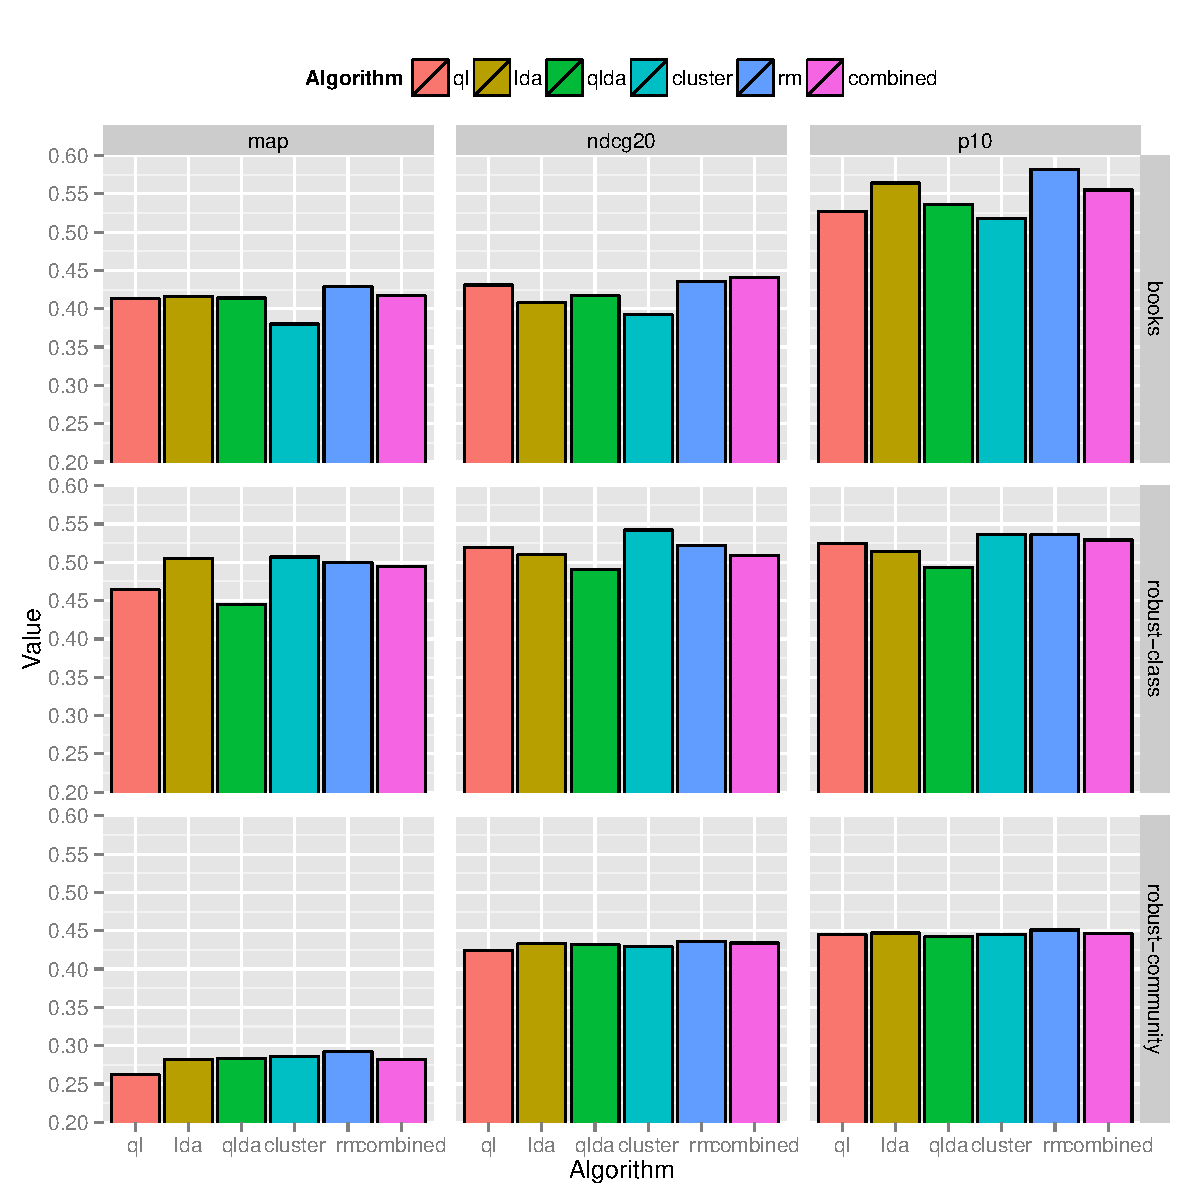
\includegraphics[width=1\textwidth]{results}}
  \caption{ql = Query Liklihood, lda = clustering using lda vectors, qlda = choose documents with most similar lda vectors to query, cluster is the clustering method from \cite{Lee2008}, rm = relevance model, and combined is clustering combining the tfidf vectors and the lda vectors.}
  \label{fig:zipf}
 \end{figure}


\begin{tabular}{cc|c|c|c|}
\cline{3-5}
& &   map & ndcg20 & p10   \\  \cline{3-5}
\hline
\multicolumn{1}{ |c  }{\multirow{6}{*}{Books} } &
\multicolumn{1}{ |c| }{Cluster} &0.3800 & 0.3920 & 0.5180   \\ \cline{2-5}
\multicolumn{1}{ |c  }{}                        &
\multicolumn{1}{ |c| }{RM} & 0.4290 & 0.4360 & 0.5820   \\ \cline{2-5}
\multicolumn{1}{ |c  }{}                        &
\multicolumn{1}{ |c| }{QL} & 0.4130 & 0.4310 & 0.5270     \\ \cline{2-5}
\multicolumn{1}{ |c  }{}                        &
\multicolumn{1}{ |c| }{LDA} & 0.4160 & 0.4080 & 0.5640    \\ \cline{2-5}
\multicolumn{1}{ |c  }{}                        &
\multicolumn{1}{ |c| }{QLDA} &0.4140 & 0.4170 & 0.5360  \\ \cline{2-5}
\multicolumn{1}{ |c  }{}                        &
\multicolumn{1}{ |c| }{Combined} & 0.4170 & 0.4410 & 0.5550     \\ \cline{1-5}

\multicolumn{1}{ |c  }{\multirow{6}{*}{Robust Class} } &
\multicolumn{1}{ |c| }{Cluster} &0.5070 & 0.5420 & 0.5360  \\ \cline{2-5}
\multicolumn{1}{ |c  }{}                        &
\multicolumn{1}{ |c| }{RM} &  0.5000 & 0.5220 & 0.5360    \\ \cline{2-5}
\multicolumn{1}{ |c  }{}                        &
\multicolumn{1}{ |c| }{QL} & 0.4640 & 0.5190 & 0.5250     \\ \cline{2-5}
\multicolumn{1}{ |c  }{}                        &
\multicolumn{1}{ |c| }{LDA} & 0.5050 & 0.5100 & 0.5140    \\ \cline{2-5}
\multicolumn{1}{ |c  }{}                        &
\multicolumn{1}{ |c| }{QLDA} & 0.4450 & 0.4910 & 0.4930    \\ \cline{2-5}
\multicolumn{1}{ |c  }{}                        &
\multicolumn{1}{ |c| }{Combined} & 0.4950 & 0.5090 & 0.5290     \\ \cline{1-5}

\multicolumn{1}{ |c  }{\multirow{6}{*}{Robust Community} } &
\multicolumn{1}{ |c| }{Cluster} & 0.2860 & 0.4290 & 0.4450   \\ \cline{2-5}
\multicolumn{1}{ |c  }{}                        &
\multicolumn{1}{ |c| }{RM} & 0.2920 & 0.4360 & 0.4510    \\ \cline{2-5}
\multicolumn{1}{ |c  }{}                        &
\multicolumn{1}{ |c| }{QL} & 0.2620 & 0.4240 & 0.4450   \\ \cline{2-5}
\multicolumn{1}{ |c  }{}                        &
\multicolumn{1}{ |c| }{LDA} & 0.2820 & 0.4330 & 0.4470    \\ \cline{2-5}
\multicolumn{1}{ |c  }{}                        &
\multicolumn{1}{ |c| }{QLDA} & 0.2830 & 0.4320 & 0.4420    \\ \cline{2-5}
\multicolumn{1}{ |c  }{}                        &
\multicolumn{1}{ |c| }{Combined} & 0.2820 & 0.4340 & 0.4460    \\ \cline{1-5}
\end{tabular}


\section {Discussion}

\bibliography{bib}
\nocite{*}
\thebibliography{bib}
\bibliographystyle{unsrt}


\end{document}